\documentclass[tikz,border=10pt]{standalone}
\usetikzlibrary{positioning, shapes.geometric, arrows.meta, calc}

\begin{document}

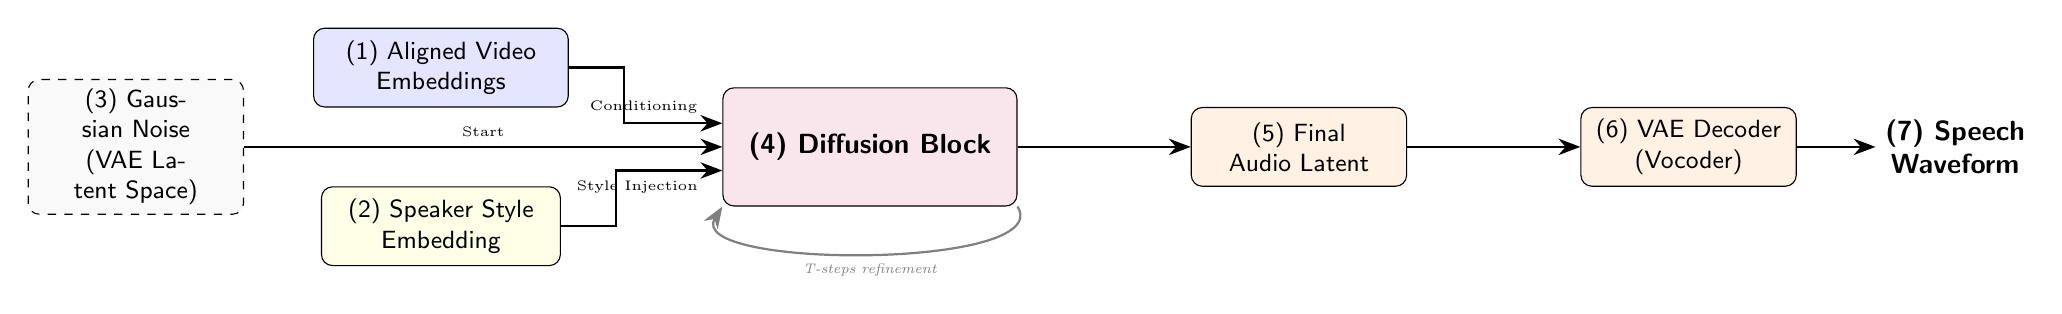
\begin{tikzpicture}[
    node distance=1.5cm and 2.2cm,
    base/.style={rectangle, draw, align=center, minimum height=1cm, font=\sffamily\small, rounded corners},
    input/.style={base, fill=gray!10, text width=2.8cm},
    proc/.style={base, fill=purple!10, text width=3.5cm, minimum height=1.5cm, font=\sffamily\bfseries},
    video_style/.style={base, fill=blue!10, text width=3cm},
    audio_style/.style={base, fill=orange!10, text width=2.5cm},
    noise_style/.style={base, fill=gray!5, dashed, text width=2.5cm},
    arrow/.style={-{Stealth[scale=1.2]}, thick}
]

    % --- INPUTS ---
    \node (video_emb) [video_style] {(1) Aligned Video\\Embeddings};
    \node (speaker_style) [input, below=1cm of video_emb, fill=yellow!10] {(2) Speaker Style\\Embedding};
    
    \node (noise) [noise_style, left=2.5cm of $(video_emb)!0.5!(speaker_style)$] {(3) Gaussian Noise\\(VAE Latent Space)};

    % --- CORE GENERATOR ---
    \node (diffusion) [proc, right=2cm of $(video_emb.east)!0.5!(speaker_style.east)$] {(4) Diffusion Block};

    % --- OUTPUT PATH ---
    \node (audio_latent) [audio_style, right=of diffusion] {(5) Final\\Audio Latent};
    \node (vae_decoder) [audio_style, right=of audio_latent] {(6) VAE Decoder\\(Vocoder)};
    \node (speech_out) [align=center, right=1cm of vae_decoder, font=\sffamily\bfseries] {(7) Speech\\Waveform};

    % --- DRAW CONNECTIONS ---
    
    % Conditioned Inputs with orthogonal paths
    \draw [arrow] (video_emb.east) -- ++(0.7,0) |- ([yshift=0.3cm]diffusion.west) 
        node[pos=0.6, above, font=\tiny] {Conditioning};
    \draw [arrow] (speaker_style.east) -- ++(0.7,0) |- ([yshift=-0.3cm]diffusion.west) 
        node[pos=0.6, below, font=\tiny] {Style Injection};

    % Noise Input
    \draw [arrow] (noise.east) -- (diffusion.west) 
        node[midway, above, font=\tiny] {Start};

    % Generation Flow
    \draw [arrow] (diffusion) -- (audio_latent);
    \draw [arrow] (audio_latent) -- (vae_decoder);
    \draw [arrow] (vae_decoder) -- (speech_out);

    % FIXED LOOP INDICATOR
    \draw [arrow, gray] (diffusion.south east) .. controls +(0.5,-0.8) and +(-0.5,-0.8) .. (diffusion.south west)
        node[midway, below, font=\tiny\itshape] {T-steps refinement};

\end{tikzpicture}

\end{document}